\chapter{Evaluation}
\label{sec:evaluation}

% Zu jeder Arbeit in unserem Bereich gehört eine Leistungsbewertung. Aus
% diesem Kapitel sollte hervorgehen, welche Methoden angewandt worden,
% die Leistungsfähigkeit zu bewerten und welche Ergebnisse dabei erzielt
% wurden. Wichtig ist es, dem Leser nicht nur ein paar Zahlen
% hinzustellen, sondern auch eine Diskussion der Ergebnisse
% vorzunehmen. Es wird empfohlen zunächst die eigenen Erwartungen
% bezüglich der Ergebnisse zu erläutern und anschließend eventuell
% festgestellte Abweichungen zu erklären.


\begin{itemize}

\item What should be evaluated
  \begin{itemize}
  \item Performance evaluation
  \item Design evaluation (lines of code, reusability)
  \item Flexibility evaluation
  \end{itemize}

\item Objective is not to implement efficient simulation, but
  it should demonstrate the developed system in its functionality
  and in comparison with MPI.

\item Own expectations
  \begin{itemize}
  \item Not much overhead compared to MPI implementation
  \item Expect the usual communication behavior
  \item less communication over network means less delay
  \item the more local calculation the more performance
  \item The software should perform as fast as the
    underlying adapter
  \end{itemize}

\item Measurements
  \begin{itemize}
  \item Configuration of the developed system (CAL, GRAPH, GVON)
  \item simulations steps per minute
  \item Idea Axel: Delay calculation of some cells
    Remap peers such that execution time of all peers
    will be the same again.
  \item Varying cluster node konfigurations
    \begin{itemize}
    \item Use different amounts of nodes
    \item Use different cluster queues
    \item Use different mapping methods
    \item Evaluate the methods and whether they
      behave like expected.
    \end{itemize}
  \end{itemize}

\item The benchmark system for evaluation was HPC system of the
  Helmholz Zentrum Dresden Rossendorf \cite{ref:hzdr_cluster}.  A part
  of the system is the hypnos linux cluster (Ubuntu 12.04.4 LTS)
  constisting of two headnodes and more than 150 compute nodes. The
  node hardware ranges from AMD Italy Opterons with two core to AMD
  Interalagos Opterons with 16 cores. Furthermore, some nodes are
  equipped with Intel Xeon CPUs with 4 cores.

  The so called laser nodes combine 4 AMD Interlagos Opterons by 4
  sockets on a single mainboard resulting in 64 CPUs per node.  The
  Interlagos Opterons 6276 are two Valencia chips on a single die,
  whereby 2 core share a 64 KByte L1 Cache and a 2 MByte L2
  Cache. Laser nodes are interconnected by an Infiniband
  network. These nodes are interesting for benchmarking, since even
  one laser node has a very complex structure

  \sitem{MPI version 1.6.3}
  \sitem{GCC 4.8.2 and application compiled with O3}


  \begin{itemize}
  \item hypnos with Linux Ubuntu 12.04.4 LTS
  \item Laser queue
    \begin{itemize}
    \item 4 sockets x 16 core AMD Opteron 6267 Interlagos = 64 core 
    \item AMD Opteron 6267 is Multi-Chip Modul (2 Valencia CPU)
    \item Nodes are connected by Infiniband
    \item 256 GB main memory
    \end{itemize}
  \item k20 queue
    \begin{itemize}
    \item 2 sockets x 4 core Xeon 2.4 GHz
    \item Nodes are connected by Infiniband
    \end{itemize}
  \item Network: Infiniband and Ethernet
  \item Communication library
  \end{itemize}
\end{itemize}

%%%%%%%%%%%%%%%%%%%%%%%%%%%%%%%%%%%%%%%%%%%%%%%%%%%%%%%%%%%%%%%%%%%%%%%%%%%%%%%%
%                                                                              %
% SYNTHETIC POINT TO POINT BENCHMARK                                           %
%                                                                              %
%%%%%%%%%%%%%%%%%%%%%%%%%%%%%%%%%%%%%%%%%%%%%%%%%%%%%%%%%%%%%%%%%%%%%%%%%%%%%%%%
\subsection{Synthetic Point to Point Benchmark}
This synthetic benchmark compares the runtime of fundamental point to
point communication operations of MPI with CAL and GVON. It is
determined the runtime overhead of CAL and GVON in respect to the
plain usage of MPI. Since this benchmark does not represent a real
world application, it does only contain communication operations of
the particular abstraction layer. Thus, the source code for the
experiments of this benchmark is free from any dependend application
logic.

Two peers are exchanging data. Whereby, one peer is the sender and the
other is the receiver. The time is measured for sending and receiving
of n messages with m elements. Such an experiment will be called
send/recv operation. Every experiment is executed 100 times and then
averaged to reduce variations in runtime. An experiment configuration
has the following parameters:

\begin{itemize}
  \item Number of consecutive send and receive operations
  \item Number of send/receive elements
  \item Communicating with and without network
  \item Selection of compute nodes kepler or laser
\end{itemize}

For the following experiments, a single parameter is variated while
the others stay fixed. This should evaluate the impact of this
parameter in respect to the MPI implementation.

\subsubsection*{Increase number of consecutive send and receive operations}
This experiment increases the number of consecutive send/recv
operations $n$ from 1 to $10^3$ by a stepsize of 10. Thereby, the amount of
sending and receiving data is set fixed to a 64 Bit integer.  The
run-time for these consecutive send/recv operations is measured and
then averaged to obtain the runtime for a single operation.  The
experiment is limited on a single node, thus, no network latency is
included in the results.  Figure \ref{fig:nsend_kepler} shows the
averaged runtime on a single kepler node and the according runtime
ration in respect to MPI.

\begin{figure}[H]
  \begin{minipage}[t]{0.5\textwidth} 
    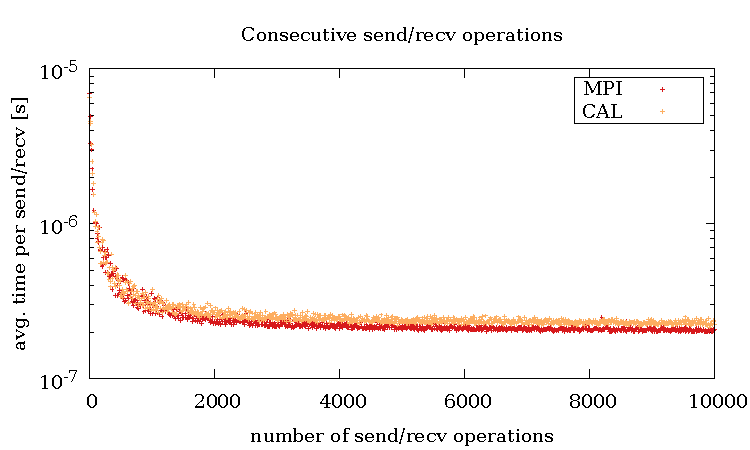
\includegraphics[width=\textwidth]{plots/50_nsend_cal_kepler}
    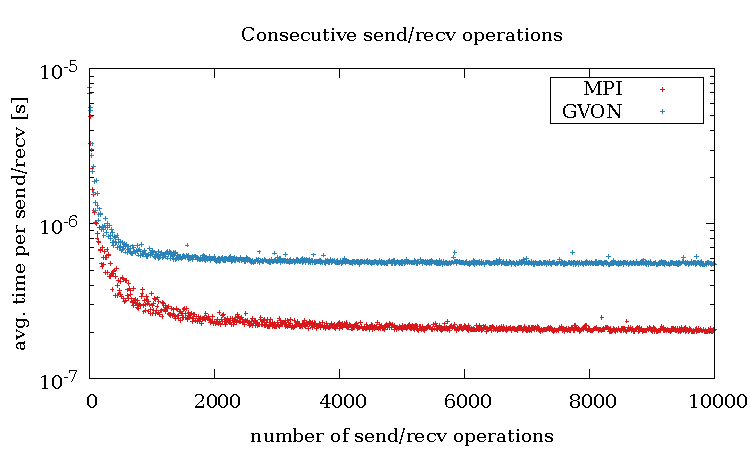
\includegraphics[width=\textwidth]{plots/50_nsend_gvon_kepler}
    \end{minipage}%
  \begin{minipage}[t]{0.5\textwidth}
    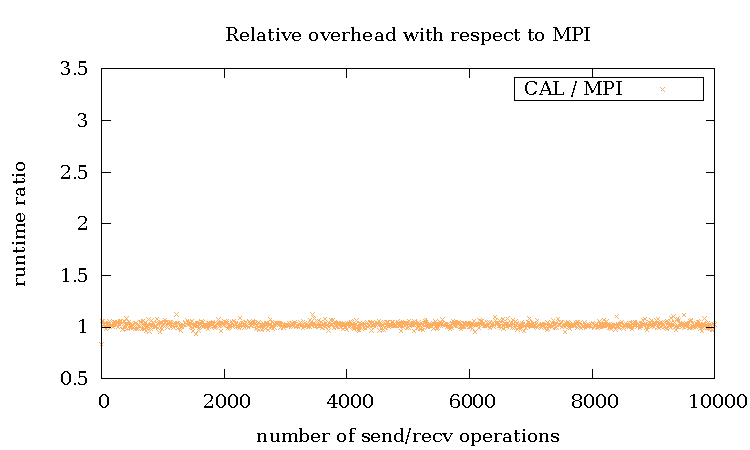
\includegraphics[width=\textwidth]{plots/50_nsend_overhead_cal}
    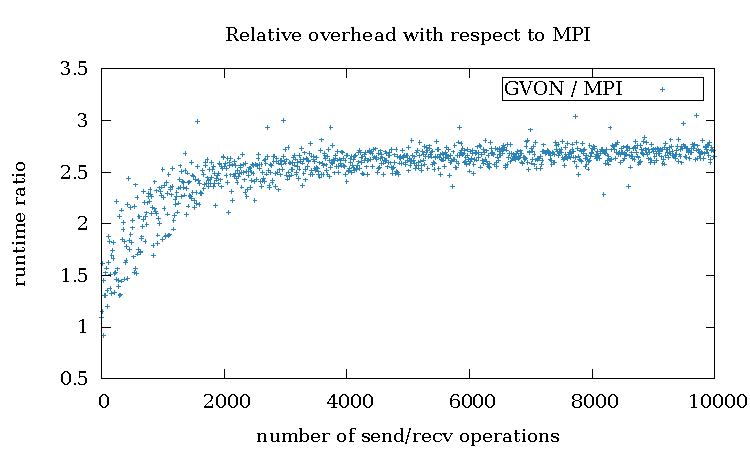
\includegraphics[width=\textwidth]{plots/50_nsend_overhead_gvon}
  \end{minipage}%
  \caption{Average run-time of a single send/recv operation and the
    according overhead of CAL and GVON compared to MPI. The number of
    consecutive operations is increased from 1 to $10^3$ by a step
    size of 10. }
  \label{fig:nsend_kepler}
\end{figure}

For both CAL and GVON, the relative overhead stabilizes with
increasing operations.  Through virtual address and context
translations, the CAL adds a constant average overhead of 10\% per
send/recv operation in respect to MPI. Even worse is the situation for
the GVON.  It adds a constant average overhead of 150\% per send/recv
operation.  Since the communication topology of the GVON is described
by a graph, including two nodes connected by a directed edge, the
constantly lookup in this graph adds constant overhead to each
send/recv operation.  Instead, CAL and MPI are sending and receiving
from fixed peer addresses. So no lookup is necessary.  However, the
graph is not changing during the experiment. Thus, it is sufficient to
perform the graph lookup only once. This should reduce the GVON
overhead to a similar level of the CAL. Figure
\ref{fig:nsend_one_lookup_kepler} shows the same experiment, but the
GVON performs only one lookup per $n$ send/recv operation.

\begin{figure}[H]
  \begin{minipage}[t]{0.5\textwidth} 
    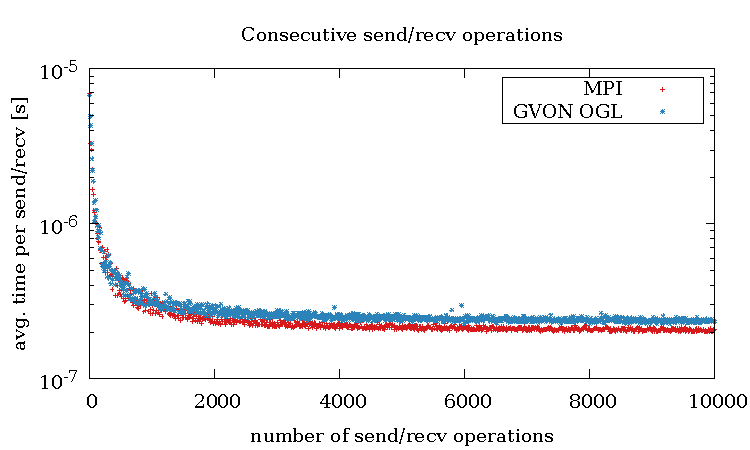
\includegraphics[width=\textwidth]{plots/50_nsend_one_lookup_kepler}
  \end{minipage}
  \begin{minipage}[t]{0.5\textwidth}
    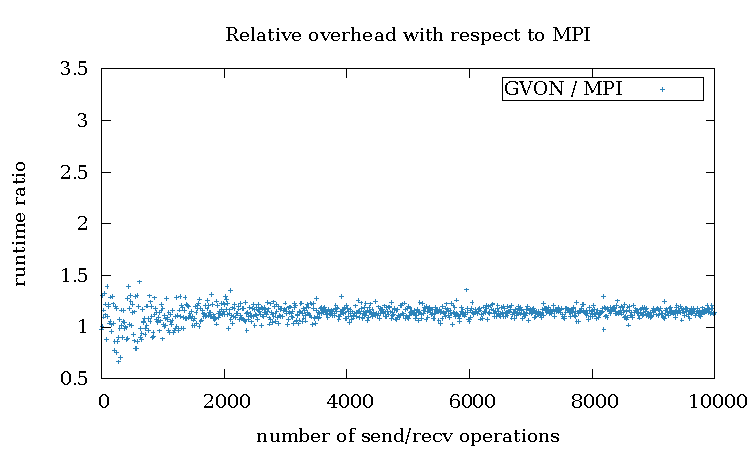
\includegraphics[width=\textwidth]{plots/50_nsend_one_lookup_overhead_gvon_kepler}
  \end{minipage}
  \label{fig:nsend_one_lookup_kepler}
  \caption{The amount of graph lookups is reduced to one lookup for
    $n$ send/recv operations.  This also reduces the GVON overhead to
    a similar level of the CAL.}
\end{figure}

\todo{Name One graph lookup, OGL}

The changed experiment reduces the GVON overhead to same level like
the CAL (around 13\%). Because the vertex and graph need to be
translated to virtual address and context, a small overhead in respect
to the CAL is still present. It shows that the graph implementation
need to be optimized with regard to lookup of incoming and outgoing
edges.

\subsubsection*{Increase number of elements per send and receive operations}
This experiment increases the number of elements per send/receive
operation from 1 to $10^3$ by a stepsize of 10. Thereby, one element is
a 64 Bit integer. A single experiment obtains the average runtime over
1000 send/receive operations.  The experiment is limited to execution
on a single node. Thus, no network latency is included in the
results. Figure \ref{fig:nsize_kepler} shows the averaged runtime of a
send/recv operation for a single element and the runtime ration in
respect to MPI.

\begin{figure}[H]
  \begin{minipage}[t]{0.5\textwidth}
    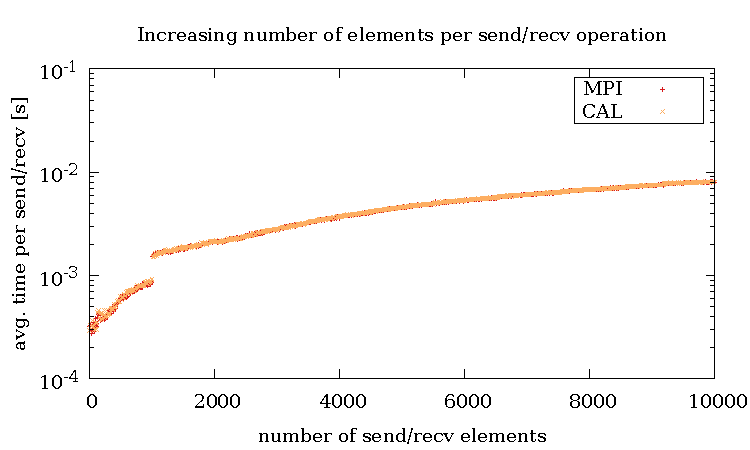
\includegraphics[width=\textwidth]{plots/50_nsize_cal_kepler}
    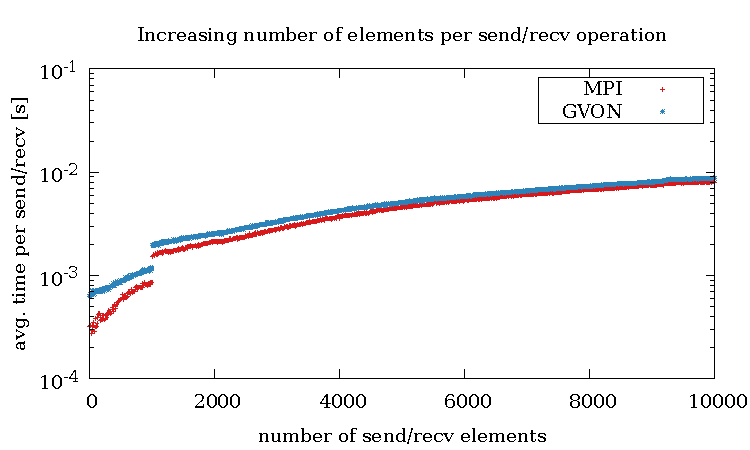
\includegraphics[width=\textwidth]{plots/50_nsize_gvon_kepler}
    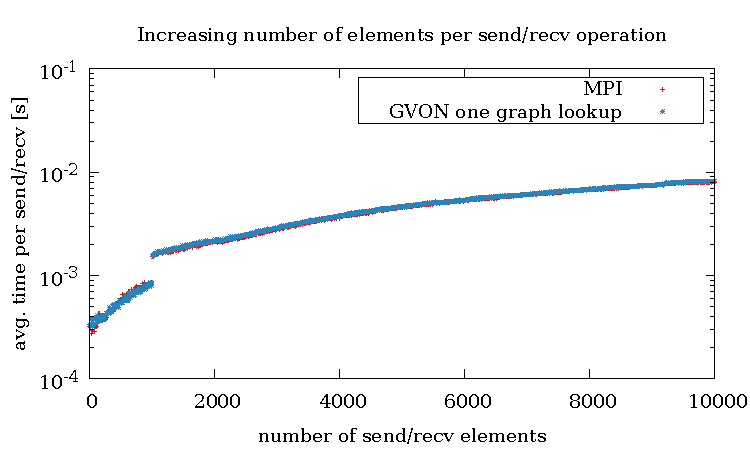
\includegraphics[width=\textwidth]{plots/50_nsize_one_lookup_gvon_kepler}
  \end{minipage}%
  \begin{minipage}[t]{0.5\textwidth}
    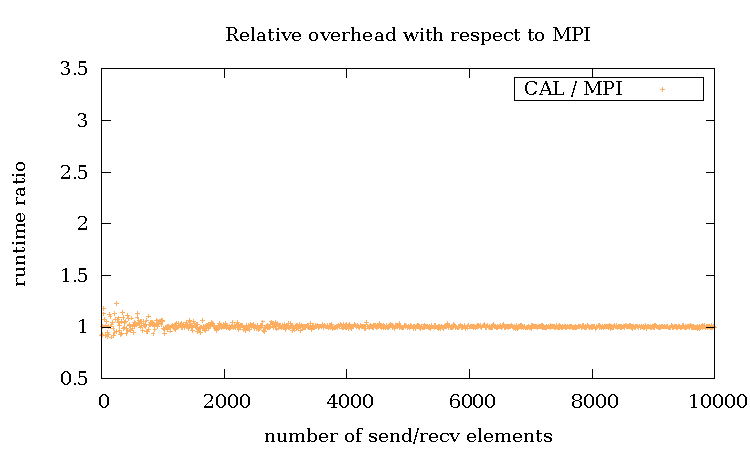
\includegraphics[width=\textwidth]{plots/50_nsize_overhead_cal_kepler}
    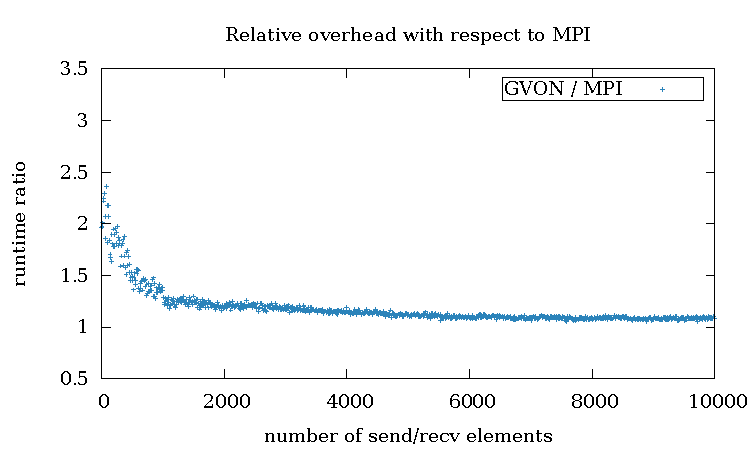
\includegraphics[width=\textwidth]{plots/50_nsize_overhead_gvon_kepler}
    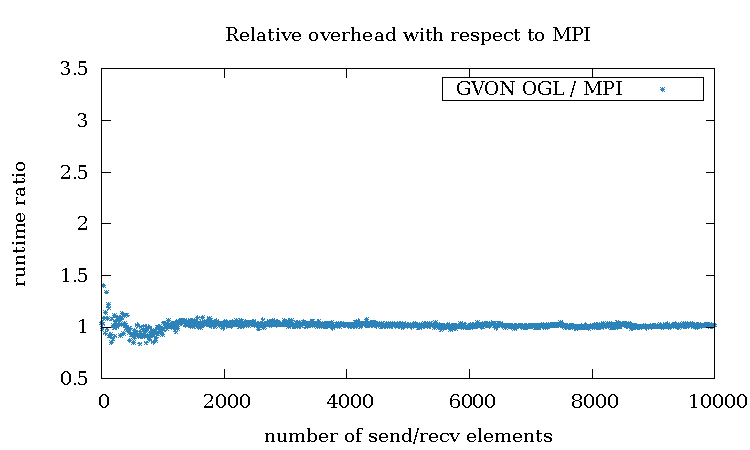
\includegraphics[width=\textwidth]{plots/50_nsize_one_lookup_overhead_gvon_kepler}
  \end{minipage}%
  \label{fig:nsize_kepler}
  \caption{Increasing the number of elements per send/recv operations, reduces
  the relative overhead in respect to MPI.}
\end{figure}

With increasing number of elements per send/recv operations the
runtime of CAL and GVON converges with MPI. The average CAL overhead
is and negligible and the average GVON overhead is reduced to only
18\% per send/recv operation. Changing the GVON experiment to a one
graph lookup variant, drops the runtime overhead even further.

\subsubsection*{Include network}
The synthetic benchmark was performed only locally on a single node
without the influence of network latency until now. The experiments
will be changed to a configuration with two nodes, whereby the peers
are not located on the same node. It is expected, that the relative
overhead of CAL and GVON decreases even more in contrast to the
previous experiments, while the overall runtime will increase.  A
setup with 8 laser nodes is used. The number of peers per node is
incremented for each experiment to a maximum of 64.

Figure
\ref{fig:nsend_network} shows the average runtime of GVON and CAL in
respect to MPI for a single send/recv operation including network
latency.

\begin{figure}[H]
  \begin{minipage}[t]{0.5\textwidth}
    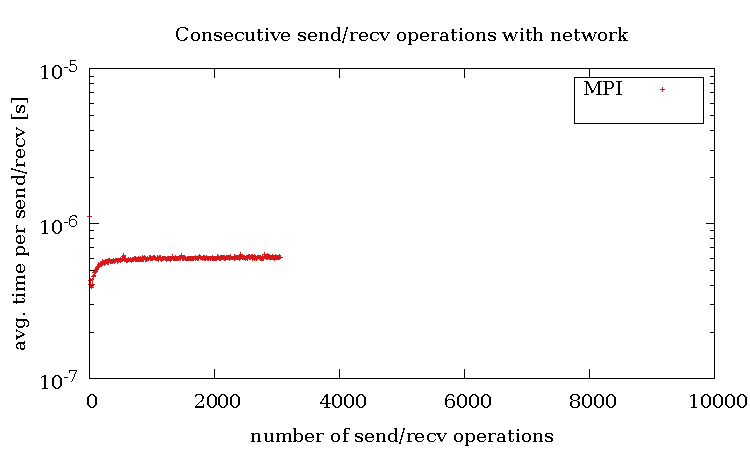
\includegraphics[width=\textwidth]{plots/50_nsend_network_cal_kepler}
    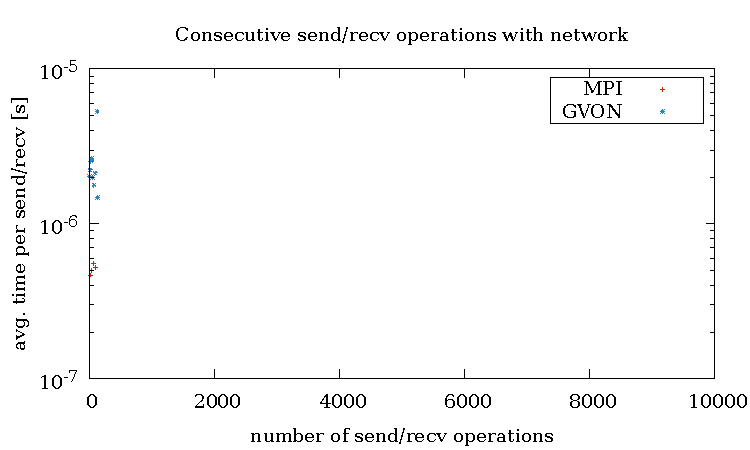
\includegraphics[width=\textwidth]{plots/50_nsend_network_gvon_kepler}
  \end{minipage}%
  \begin{minipage}[t]{0.5\textwidth}
    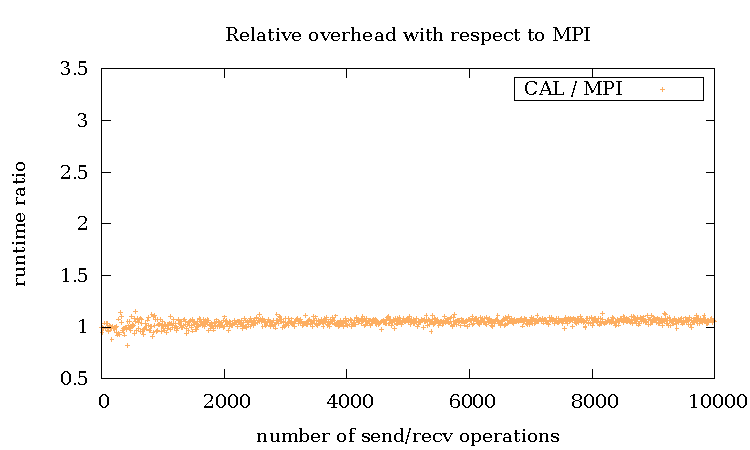
\includegraphics[width=\textwidth]{plots/50_nsend_network_overhead_cal_kepler}
    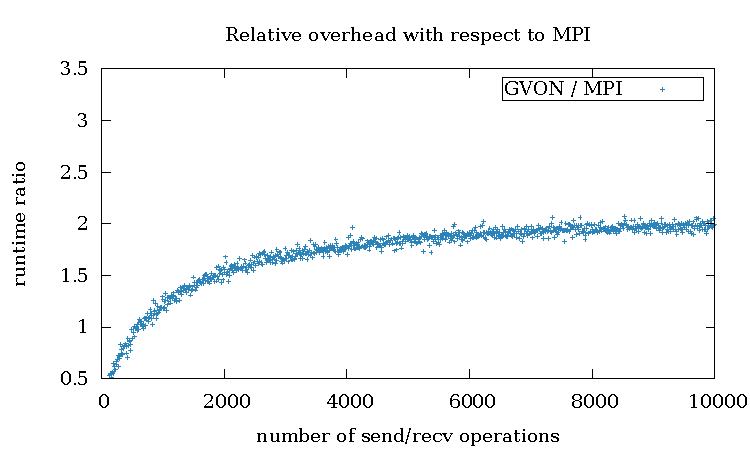
\includegraphics[width=\textwidth]{plots/50_nsend_network_overhead_gvon_kepler}
  \end{minipage}%
  \caption{ }
  \label{fig:nsend_network}

\end{figure}



%%%%%%%%%%%%%%%%%%%%%%%%%%%%%%%%%%%%%%%%%%%%%%%%%%%%%%%%%%%%%%%%%%%%%%%%%%%%%%%%
%                                                                              %
% SYNTHETIC COLLECTIVE BENCHMARK                                               %
%                                                                              %
%%%%%%%%%%%%%%%%%%%%%%%%%%%%%%%%%%%%%%%%%%%%%%%%%%%%%%%%%%%%%%%%%%%%%%%%%%%%%%%%
\subsection{Synthetic Collective Benchmark}
This benchmark compares the runtime of MPI collective operations with
collevtives of CAL and GVON.  Thereby, to determine the runtime for a
single collective execution, it is executed 1000 times and then
averaged. Since, the overhead in respect to MPI should be determined,
only the gather and reduce collective were chosen for comparison.

\begin{itemize}
\item Synthetic Collective Tests
  \begin{itemize}
  \item GVON only implements gather and reduce
  \item N collective operations
  \item average runtime of one collective operation
  \item Increase amount of data to send
  \item Varying data types
  \item Compare MPI, CAL, GVON
  \end{itemize}

\end{itemize}


\subsubsection*{Gather Collective}

\begin{itemize}
  \item CAL and MPI collectives are quiete similar
  \item GVON executes collective operations locally first
  \item GVON does reordering of collective results
  \item Big relative overhead is expected
\end{itemize}

Figure \ref{fig:collective_npeers} shows the average runtime of a
gather collective for increasing number of peers.

\begin{figure}[H]
  \begin{minipage}[t]{0.5\textwidth}
  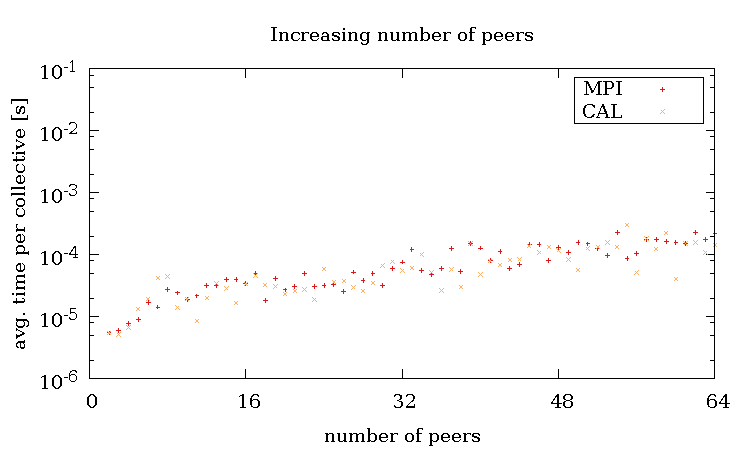
\includegraphics[width=\textwidth]{plots/50_collective_npeers_cal_laser}
  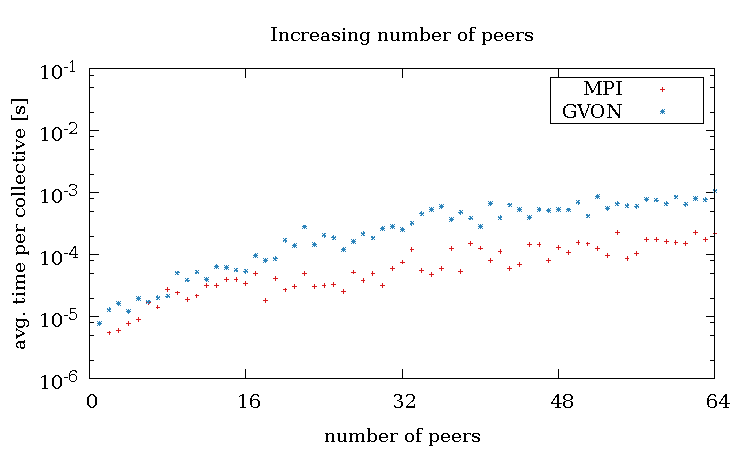
\includegraphics[width=\textwidth]{plots/50_collective_npeers_gvon_laser}
  \end{minipage}%
  \begin{minipage}[t]{0.5\textwidth}
  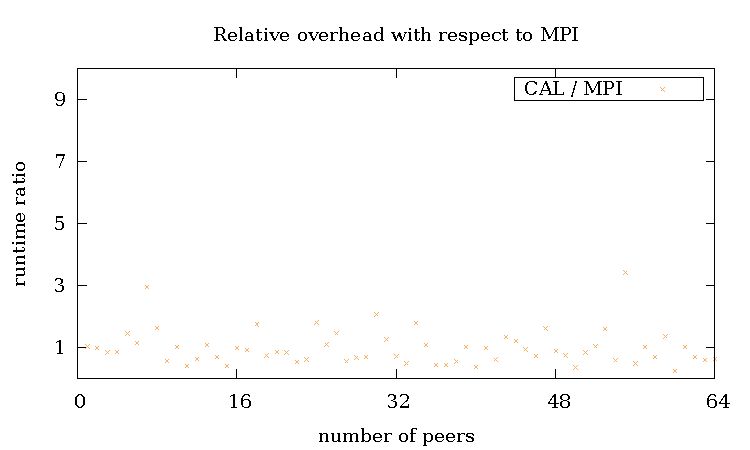
\includegraphics[width=\textwidth]{plots/50_collective_npeers_overhead_cal_laser}
  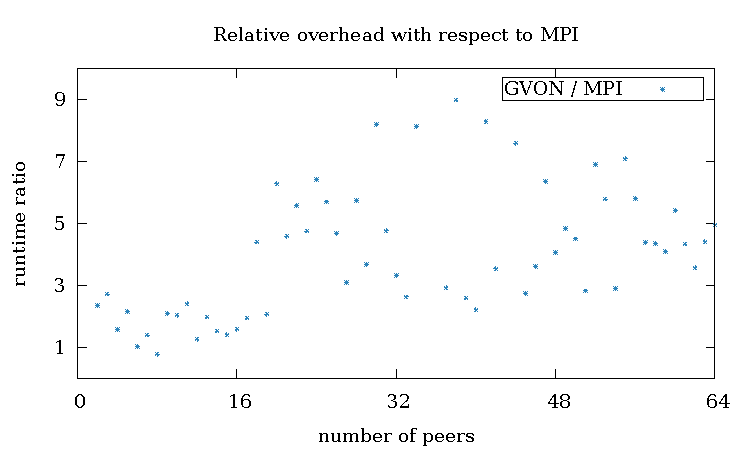
\includegraphics[width=\textwidth]{plots/50_collective_npeers_overhead_gvon_laser}
  \end{minipage}%
  \caption{ }
  \label{fig:collective_npeers}
\end{figure}


\todo{include network}

\subsubsection*{Reduce Collective}




%%%%%%%%%%%%%%%%%%%%%%%%%%%%%%%%%%%%%%%%%%%%%%%%%%%%%%%%%%%%%%%%%%%%%%%%%%%%%%%%
%                                                                              %
% GAME OF LIFE BENCHMARK                                                       %
%                                                                              %
%%%%%%%%%%%%%%%%%%%%%%%%%%%%%%%%%%%%%%%%%%%%%%%%%%%%%%%%%%%%%%%%%%%%%%%%%%%%%%%%
\subsection{Game of Life Benchmark}
The previous benchmarks evaluated the developed system in a very
synthetic and unreal manner. But, real world simulation perform
calculations in between communication operations. The Game of Life
simulation should be an example for such an real world
simulation. Therefore, this benchmark compares the presented GoL
implementation with an equivalent MPI implementation. Equivalent
refers to the same set of rules, the same amount of communication
operations and the same functions are used to update the cell states.
The GoL domain is square field with $n^2$ cells and the state of every
cell is calculated by a peer.  Figure \ref{fig:gol_laser} shows the
average run-time of a time-step for $n$ in range from 1 to 8. The
Experiment is limited to a single laser node.

\begin{figure}[H]
  \begin{minipage}[t]{0.5\textwidth}
    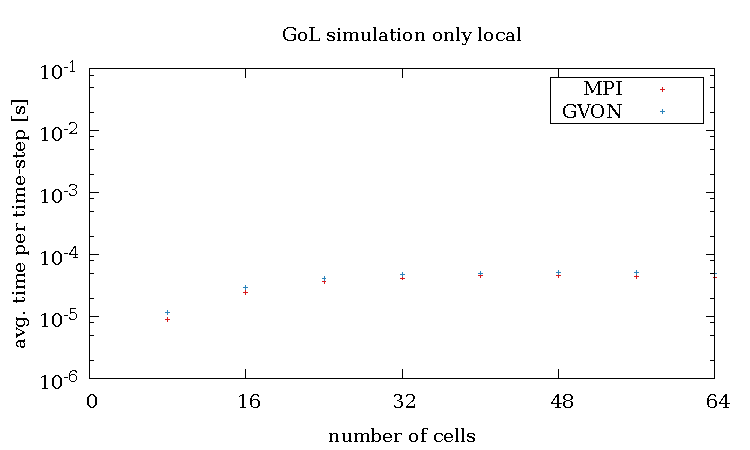
\includegraphics[width=\textwidth]{plots/50_gol_ncells_laser}
    \label{fig:gol_laser}
    \caption{ }
  \end{minipage}%
  \begin{minipage}[t]{0.5\textwidth}
    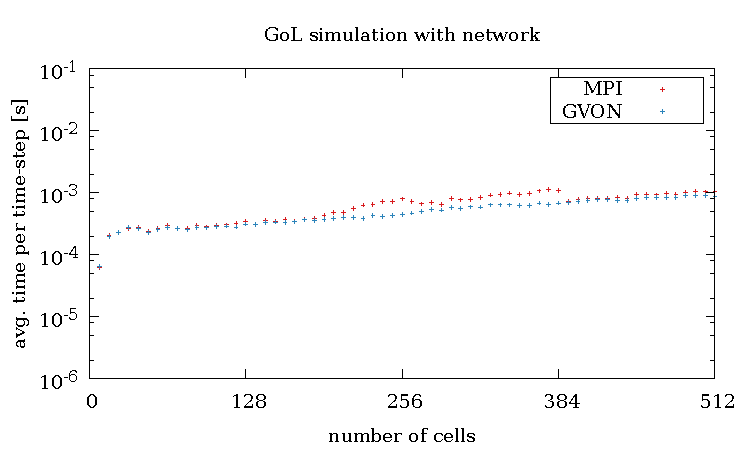
\includegraphics[width=\textwidth]{plots/50_gol_network_laser}
    \label{fig:gol_network_laser}
    \caption{ }
  \end{minipage}%
\end{figure}

The peers are equally distributed to 8 laser nodes. Figures
\ref{fig:gol_network_laser} shows the average run-time of a time-step
for $n$ in range from 1 to 22.

\subsubsection*{Including Network}

%%%%%%%%%%%%%%%%%%%%%%%%%%%%%%%%%%%%%%%%%%%%%%%%%%%%%%%%%%%%%%%%%%%%%%%%%%%%%%%%
%                                                                              %
% N BODY BENCHMARK                                                             %
%                                                                              %
%%%%%%%%%%%%%%%%%%%%%%%%%%%%%%%%%%%%%%%%%%%%%%%%%%%%%%%%%%%%%%%%%%%%%%%%%%%%%%%%
\subsection{N Body Benchmark}
This benchmark simulates the implemented n body simulation for 1000
time-steps with increasing number of bodies. It is compared a
simulation implemented with MPI to one implemented with the GVON. In
contrast to the synthetic benchmark, calculations have to be performed
in between communication operations. Thus, the communication operations
do not provide the main run-time. Figure \ref{fig:nbody_laser} shows
the averaged run-time of a time-step with increasing number of bodies.

\begin{figure}[H]
  \begin{minipage}[t]{0.5\textwidth}
   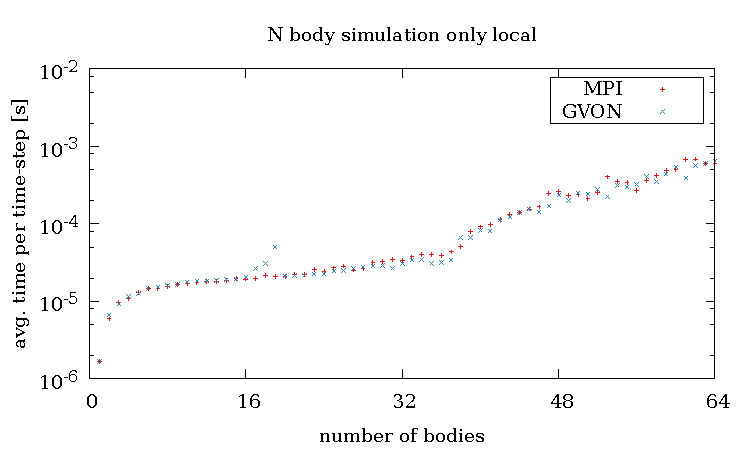
\includegraphics[width=\textwidth]{plots/50_nbody_laser}
  \label{fig:nbody_laser}
  \caption{ }
  \end{minipage}%
  \begin{minipage}[t]{0.5\textwidth}
    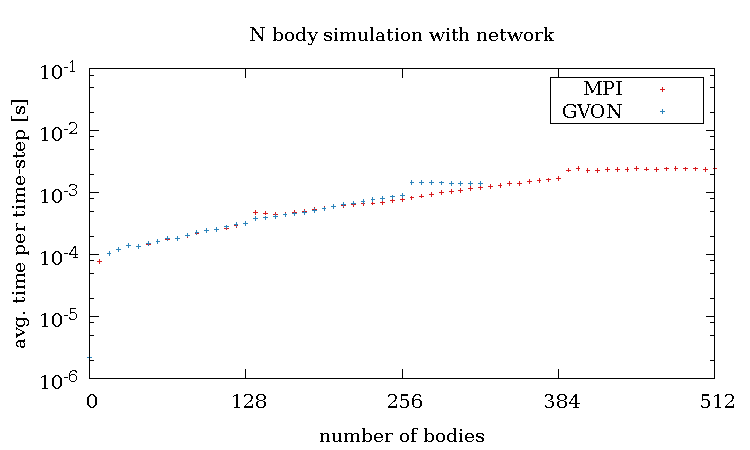
\includegraphics[width=\textwidth]{plots/50_nbody_network_laser}
    \label{fig:nbody_network_laser}
    \caption{ }
  \end{minipage}%
\end{figure}

The average run-time of a time-step raises quadratic with the number
of bodies. Also the variance increases quadratic. Thus, the run-time
of the time-steps varies strongly.

\sitem{Still no explanation for strong variance}


\begin{itemize}
  \item Simple N-Body
    \begin{itemize}
    \item 1 to 256 Bodies
    \item runs on laser machine (64 CPU's)
    \item run of 1000 time-steps
    \item max 4 bodies per CPU
    \item Compare with and without network
    \item Compare MPI with GVON
    \item Compare different amount of CPU's
    \end{itemize}
\end{itemize}

\subsubsection*{Including Network}


%%%%%%%%%%%%%%%%%%%%%%%%%%%%%%%%%%%%%%%%%%%%%%%%%%%%%%%%%%%%%%%%%%%%%%%%%%%%%%%%
%                                                                              %
% CONCLUSION                                                                   %
%                                                                              %
%%%%%%%%%%%%%%%%%%%%%%%%%%%%%%%%%%%%%%%%%%%%%%%%%%%%%%%%%%%%%%%%%%%%%%%%%%%%%%%%
\begin{itemize}
\item Conclusion about evaluation points. What can
  be done better, where can the system be changed.
  Give reason for behavior of the system.

\end{itemize}

\cleardoublepage

%%% Local Variables:
%%% TeX-master: "diplom"
%%% End:
